%%%%%%%%%%%%%%%%%%%%%%%%%%%%%%%%%%%%%%%%%%%%%%%%%%%%%%%
\mychapter{Exames com Quadro de Respostas (QR)}\label{ch:examesQR}

Este capítulo se concentra na criação de exames que exclusivamente apresentam o quadro de resposta (QR). Essa abordagem é particularmente útil quando os enunciados das questões são fornecidos separadamente. É uma prática amplamente adotada na Escola Preparatória da UFABC (EPUFABC) para processos seletivos e simulados que envolvem inúmeros estudantes anualmente.

Será demonstrado como acomodar centenas de questões em uma única página em formato PDF, que pode ser impressa e distribuída aos estudantes para preencherem manualmente as respostas. Posteriormente, os QRs são digitalizados e enviados ao MCTest para correção. O sistema encaminha ao professor um e-mail contendo arquivos CSV com as marcações de cada estudante e as respostas corretas. Além disso, em poucos minutos, o MCTest fornece uma síntese da Teoria de Respostas ao Item (TRI) com base nas correções realizadas, a menos que ocorra algum erro no processo de correção, como a não decodificação do QRCode.

O gabarito, ou seja, as respostas corretas, é disponibilizado na primeira página do PDF digitalizado, que pode conter as respostas de todos os estudantes de uma turma em sequência.

\section{Utilizando exames exclusivamente com QR}\label{sec:examesQR}

Conforme visto no capítulo anterior, na Seção \ref{sec:telaExame} -- \nameref{sec:telaExame}, ao criar um exame, a configuração padrão é para um exame com exclusivamente o QR, como mostrado na Figura \ref{fig:cap06_figExamePDF_QRpadrao}. Para esse estilo de exame, o professor só precisa selecionar a(s) turma(s) e seguir as instruções descritas na Seção \ref{sec:exameDetalhes} -- \nameref{sec:exameDetalhes} para configurar os detalhes do exame. Nesse caso, é necessário definir o número de questões em uma escala de dificuldade de 1 a 5 e o número de alternativas de cada questão na parte esquerda da Figura \ref{fig:cap06_figExameAtualizaConfiguracoes}. Na parte direita, você deve informar a quantidade de questões por bloco/quadro e escolher a quantidade de blocos por linha, além de definir se o estilo do exame será horizontal ou vertical. Certifique-se de marcar as opções ``Questões/Respostas/Ambos=Respostas'', ``Ecológico=Sim'' e ``Retorno=Não''. As instruções do exame podem ser definidas no campo ``Instruções'' e é possível utilizar a formatação de itens com o comando \verb|\item|. 

\subsection{Estilo vertical}

Na Figura \ref{fig:cap07_figvertical}, é apresentado um recorte do cabeçalho do exame, que inclui os dados do candidato e o QR. No processo seletivo da EPUFABC, realizado em 2019, houve a digitalização de 2553 QRs. Nesse caso específico, foi adotado o estilo vertical, com 25 questões por bloco e dois blocos por linha. Observa-se no cabeçalho a presença de um QRcode (\textit{Quick Response Code}) criptografado e compactado, contendo informações do exame e do candidato. Apenas 13 exames tiveram o código não reconhecido (normalmente, basta digitalizá-lo novamente com uma resolução melhor para funcionar). Além disso, somente 5 candidatos preencheram o QR incorretamente. Por exemplo, na Figura \ref{fig:cap07_figvertical}, é possível observar que o candidato ultrapassou o local de marcação na questão 48. Quando isso acontece, é possível corrigir a marcação errada utilizando um corretivo ou um editor de PDF que permite a edição de imagens no próprio documento, como o site \href{https://www.ilovepdf.com/pt/editar-pdf}{ilovepdf.com}. No entanto, é importante ter cuidado para não remover parte dos círculos ao realizar a correção.

\begin{figure}[htbp]
  \centering
  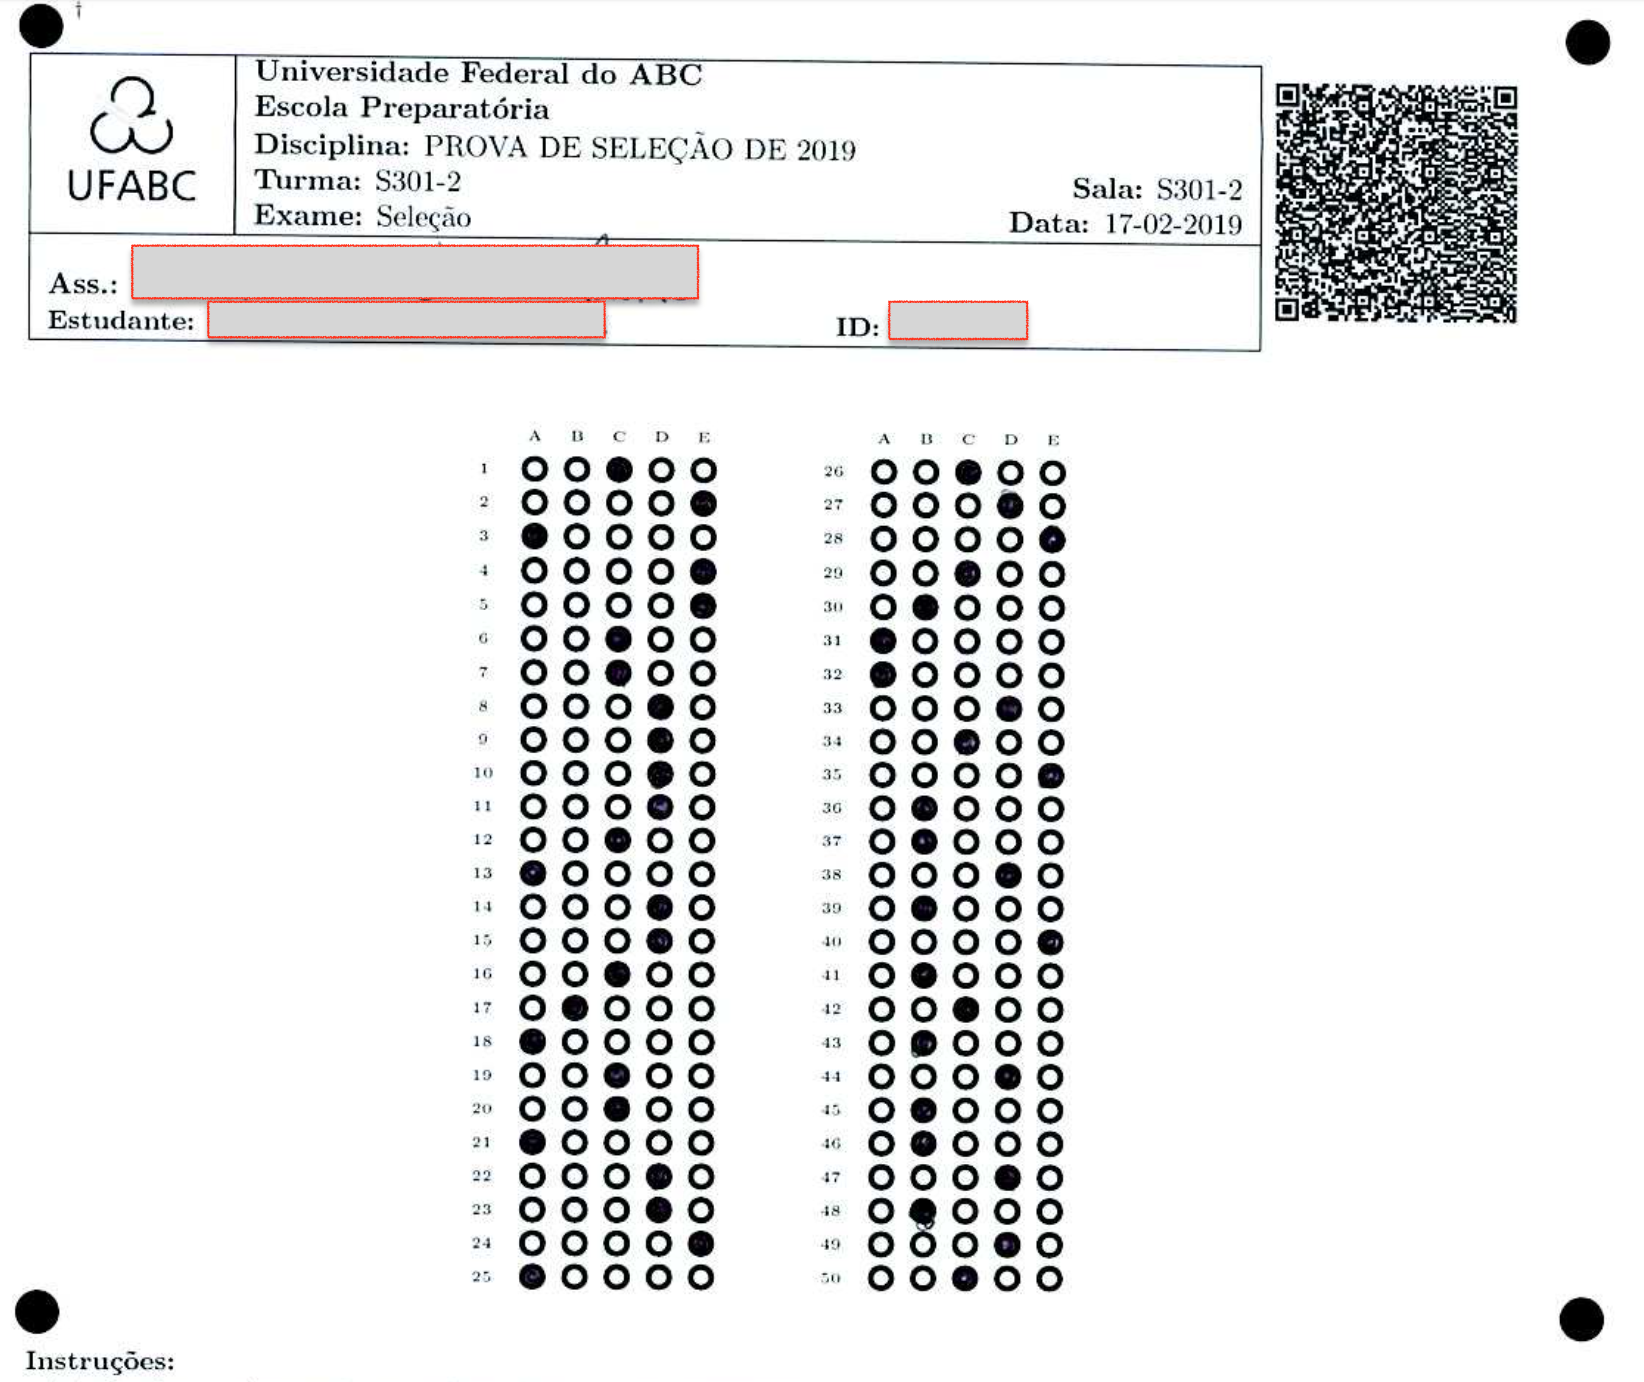
\includegraphics[width=0.9\textwidth]{cap07_figvertical.png}
    \caption{Recorte de um exame digitalizado em formato PDF no estilo vertical.}
 \label{fig:cap07_figvertical}
\end{figure}

Um exemplo de instruções, que contou com a colaboração do Prof. Dr. Leonardo Steil, então Pró-Reitor de Extensão, para redigir o texto, é mostrado na Figura \ref{fig:cap07_figinstrucoes}, utilizado no processo seletivo de 2019 da EPUFABC.

\begin{figure}[htbp]
  \centering
  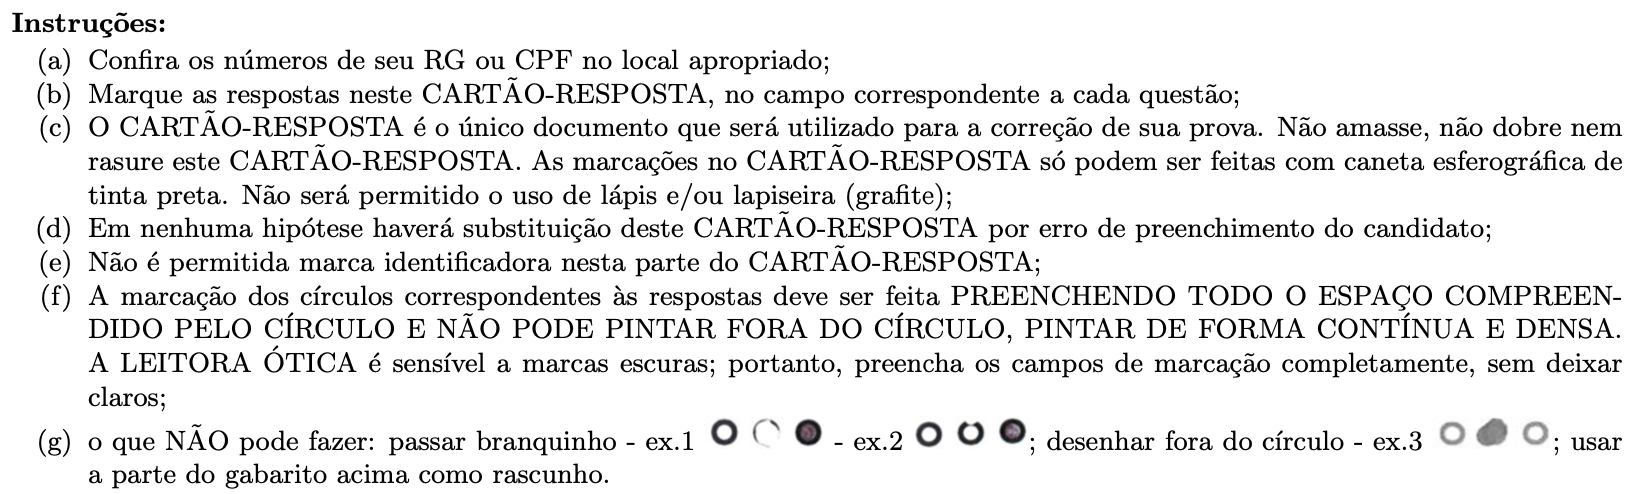
\includegraphics[width=0.9\textwidth]{cap07_figinstrucoes.png}
    \caption{Recorte de um exame em formato PDF no estilo vertical, com as instruções.}
 \label{fig:cap07_figinstrucoes}
\end{figure}

Com esse exemplo realizado na EPUFABC, foi destacada a utilidade do MCTest na realização de avaliações para inúmeros estudantes. No caso em questão, foi criado um único arquivo CSV para preencher as 29 turmas, uma em cada sala de aula, conforme descrito na Seção \ref{sec:variasTurmasCSV} - \textit{\nameref{sec:variasTurmasCSV}}. Em seguida, foi configurado um único exame selecionando todas as turmas e gerados os PDFs, um por turma, conforme detalhado na Seção \ref{sec:exameRecorte1} - \textit{\nameref{sec:exameRecorte1}}. Os exames foram impressos e aplicados aos estudantes. Posteriormente, foi realizada a digitalização dos QRs, conforme explicado na Seção \ref{sec:exameRecorte1}. O MCTest então enviou as correções dos exames. Em casos em que ocorreu algum erro durante o processo de correção do QR, uma imagem da questão e das alternativas foi salva e incluída em um arquivo ZIP que também foi enviado ao professor por e-mail.

\subsection{Estilo horizontal}

Para minimizar os erros nas marcações dos círculos, foi desenvolvido o estilo horizontal, como ilustrado na Figura \ref{fig:cap07_fighorizontal}. É importante observar que, na questão 15 desta figura, o candidato utilizou corretivo, o que impossibilitou o algoritmo de visão computacional de corrigir automaticamente esse exame. Esse estilo foi aplicado no processo seletivo da EPUFABC em 2020, com 2053 exames digitalizados, 3 QRCodes não identificados e apenas uma falha nas correções das respostas, conforme mostrado na Figura \ref{fig:cap07_fighorizontal}. Além disso, o estilo horizontal ocupa menos espaço na folha de exame, o que é especialmente útil quando se deseja incluir tanto o QR quanto as questões em uma única folha, como utilizado no processo seletivo da Especialização em Tecnologias e Sistemas da Informação (TSI), que será apresentado no próximo capítulo.

\begin{figure}[htbp]
  \centering
  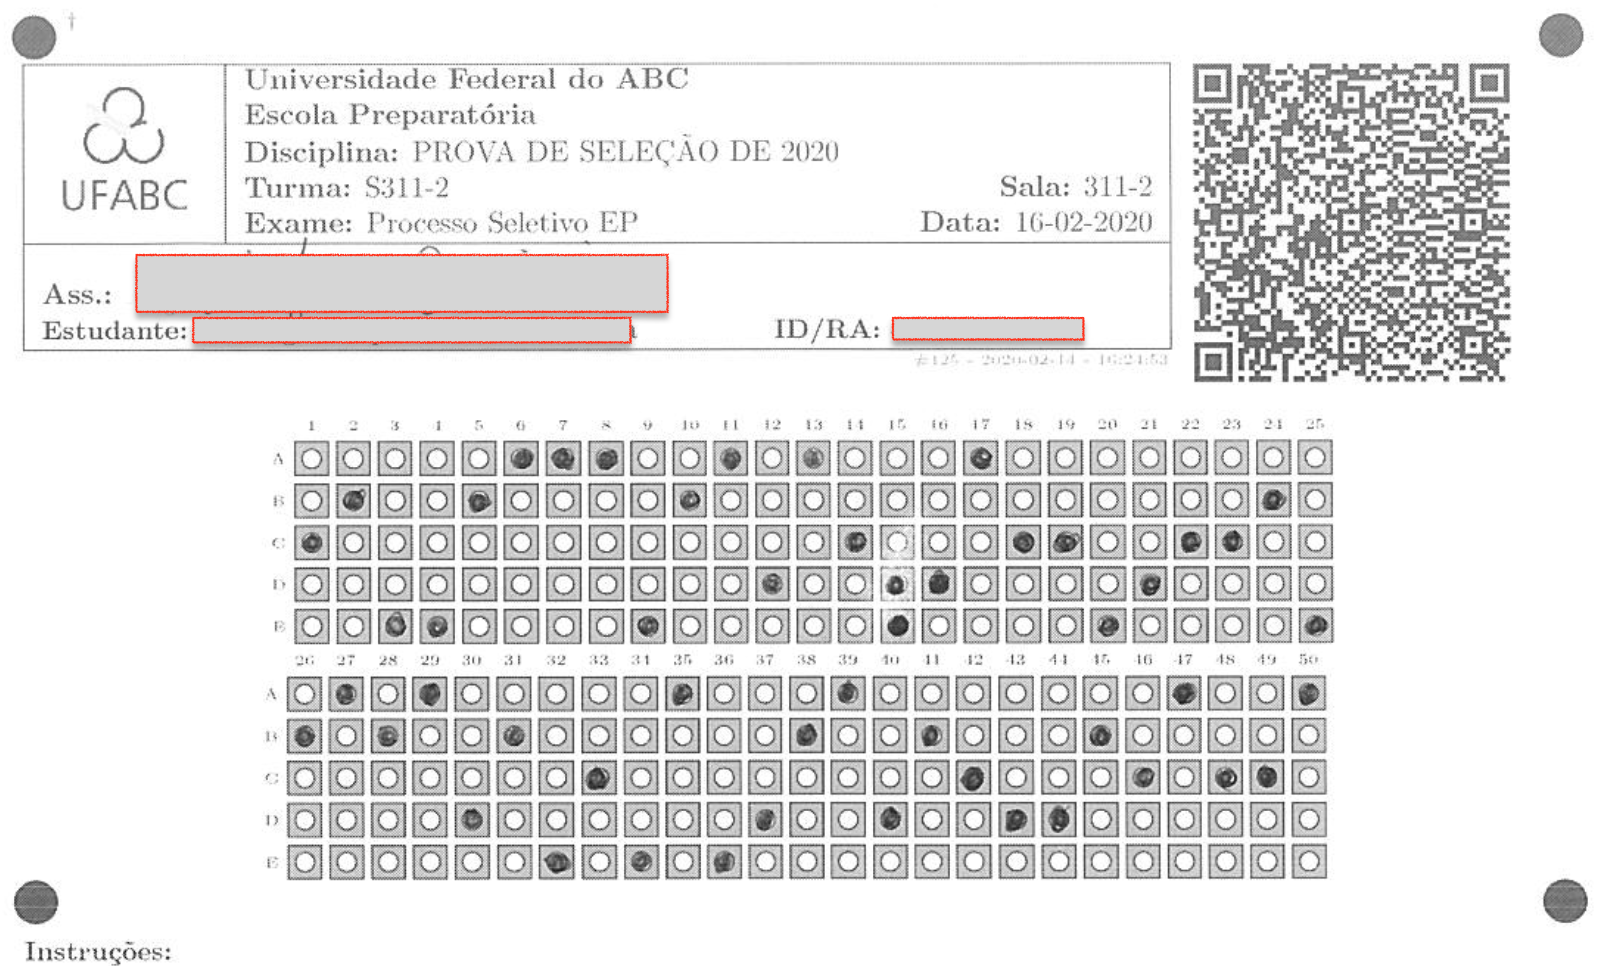
\includegraphics[width=0.9\textwidth]{cap07_fighorizontal.png}
    \caption{Recorte de um exame digitalizado em formato PDF no estilo horizontal.}
 \label{fig:cap07_fighorizontal}
\end{figure}

O restante deste capítulo fornecerá mais detalhes sobre esse estilo de exame que inclui exclusivamente o QR.

\section{Restrições nos QRs}

Na Figura \ref{fig:cap07_figmaxVertigal}, são apresentados exemplos de exames com a quantidade máxima de questões nos estilos horizontal (245 questões) e vertical (200 questões). É importante ressaltar que, se o número de alternativas for menor do que cinco, esses valores máximos serão ainda maiores. \textbf{O número mínimo de alternativas permitidas por questão é três}. Além disso, é relevante destacar que apenas a página da frente pode ser utilizada para a construção dos QRs.


\begin{figure}[htbp]
\centering
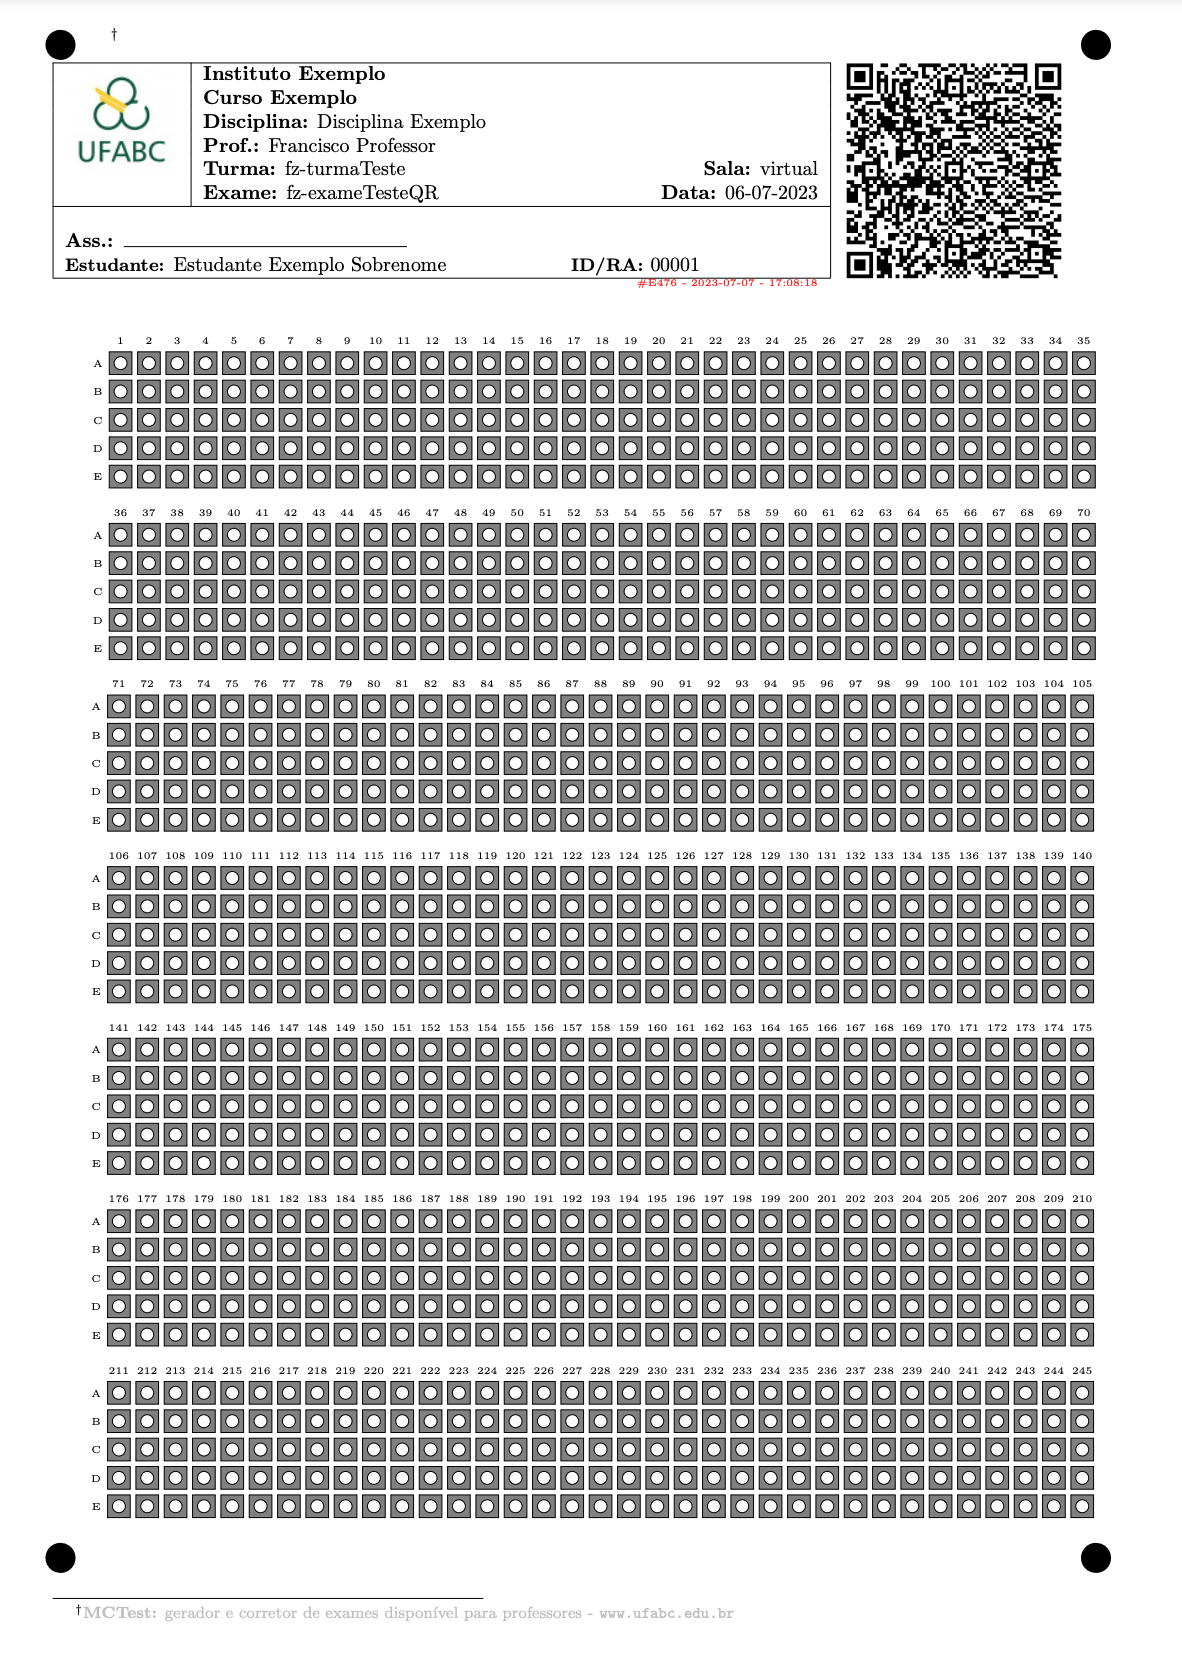
\includegraphics[width=0.49\textwidth]{cap07_figmaxHorizontal.png}
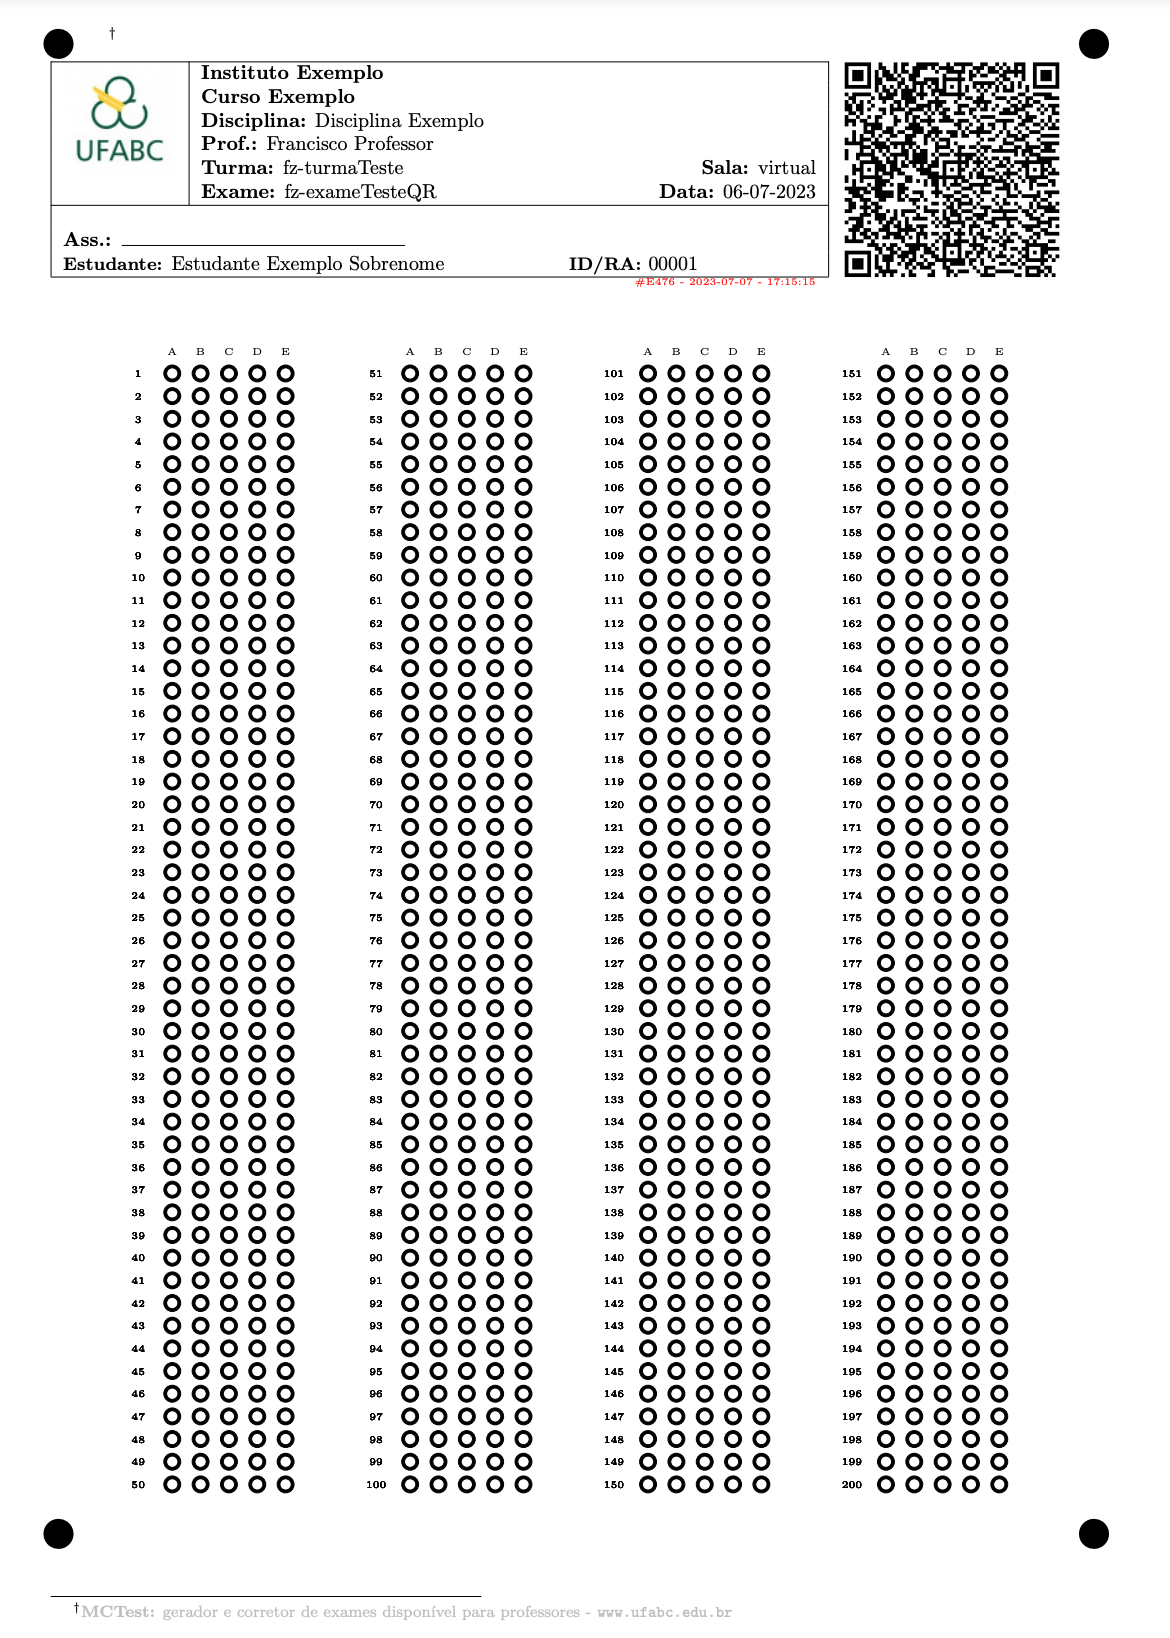
\includegraphics[width=0.49\textwidth]{cap07_figmaxVertigal.png}
\caption{Exemplos de PDFs de exames com 245 questões no estilo horizontal e 200 questões no estilo vertical.}
\label{fig:cap07_figmaxVertigal}
\end{figure}

A seguir, serão apresentadas mais restrições relacionadas à organização dos QRs. \textbf{O número mínimo de questões por bloco é três}. Portanto, se for criado um exame com 17 questões, cinco questões por bloco e dois blocos por linha, ocorrerá um erro, pois não é possível ter um bloco com apenas duas questões. Uma alternativa nesse caso seria criar blocos com seis questões cada um, por exemplo. Na Figura \ref{fig:cap07_figquestoesPorBloco}, é mostrado um exemplo contendo 18 questões, cinco questões por bloco e dois blocos por linha.



\begin{figure}[htbp]
\centering
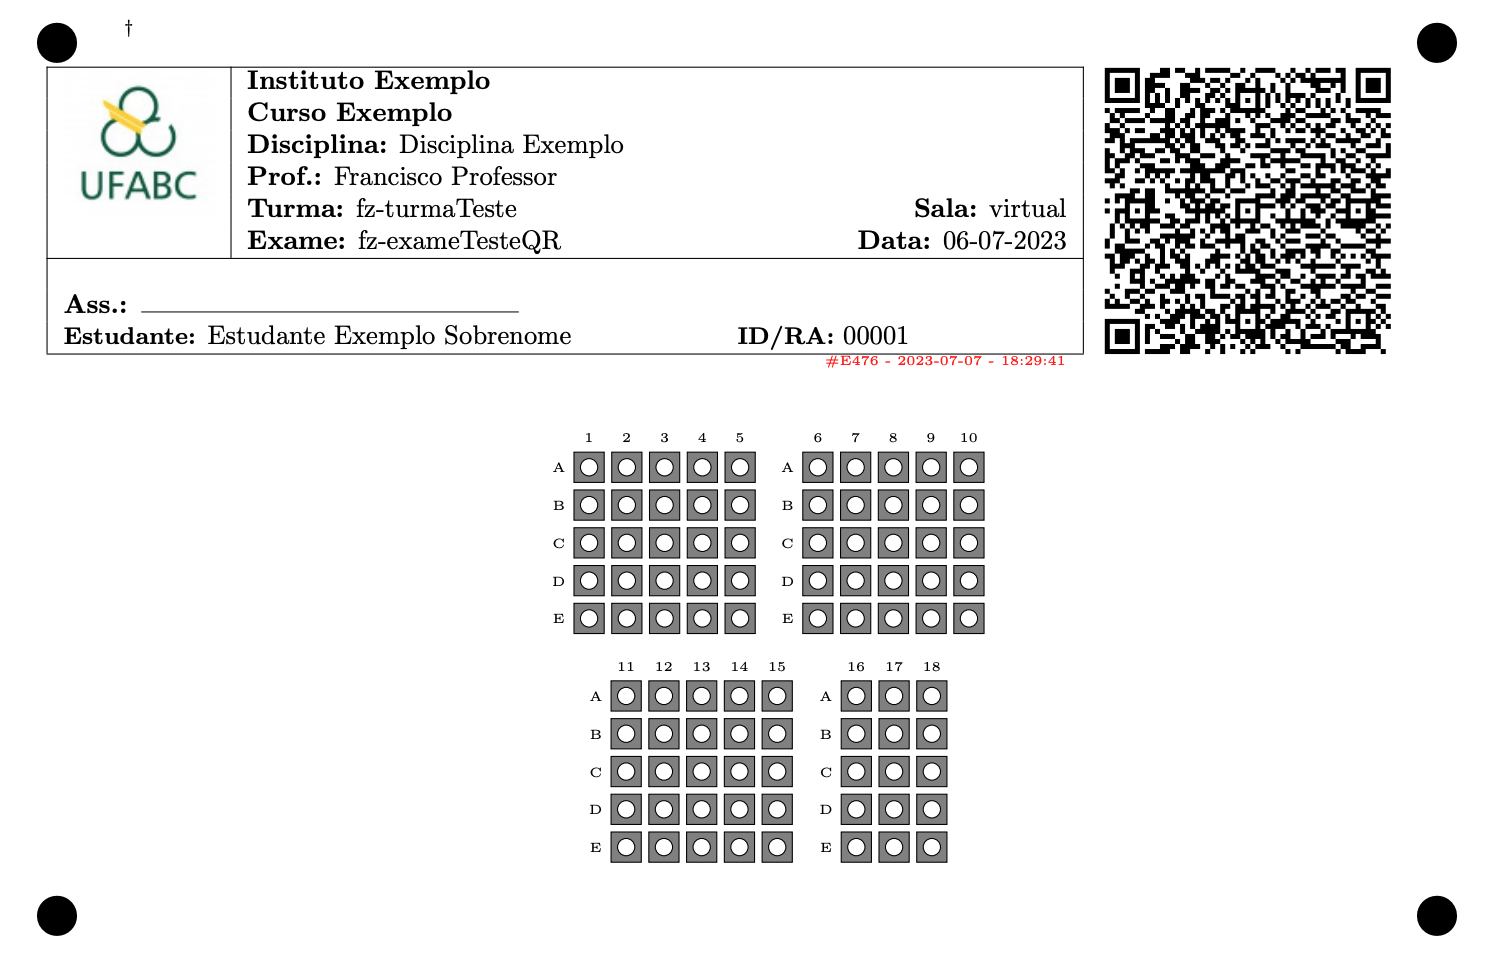
\includegraphics[width=0.9\textwidth]{cap07_figquestoesPorBloco.png}
\caption{Exemplo de PDF de um exame com 18 questões, cinco questões por bloco e dois blocos por linha.}
\label{fig:cap07_figquestoesPorBloco}
\end{figure}

%%%%%%%%%%%%%%%%%%%%%%%%%%%%%%%%%%%%%%%%%%%%%%%%%%%%%%%%%%%%%%%%%%%%
\section{Corrigindo exames com QR}\label{sec:examesCorrigirQR}

Foi criado um PDF destinado a uma turma com três estudantes, sendo o primeiro exclusivamente para armazenar o gabarito, conforme ilustrado na Figura \ref{fig:cap07_figquestoesPorBloco}. Após a impressão desse PDF, o gabarito foi preenchido e digitalizado, como mostrado na Figura \ref{fig:cap07_figquestoesPorBlocoScan}--(a). Em seguida, mais dois QRs foram preenchidos e digitalizados, conforme apresentado nas Figuras \ref{fig:cap07_figquestoesPorBlocoScan}--(b) e (c). Todas as três digitalizações foram armazenadas em um único PDF, sendo a primeira página estritamente destinada ao gabarito.

No segundo QR, Figura \ref{fig:cap07_figquestoesPorBlocoScan}--(b), optou-se por introduzir vários erros no preenchimento das alternativas nos terceiro e quarto blocos; os detalhes estão disponíveis na Figura \ref{fig:cap07_figquestoesPorBlocoScanErros}. Nesse caso específico, os erros foram gerados intencionalmente ao marcar mais de uma alternativa em algumas questões, para avaliar a capacidade do método de visão computacional em detectar essas marcações incorretas. 

Na terceira página do PDF, Figura \ref{fig:cap07_figquestoesPorBlocoScan}--(c), decidiu-se repetir o gabarito para simular um estudante que obteve a nota máxima nesta avaliação. No entanto, a questão 9 não foi considerada devido à marcação insuficiente. 

O algoritmo implementado para considerar uma marcação correta exige que mais de 50\% da área esteja marcada dentro do círculo. Se houver mais de uma marcação, em alguns casos, é considerada a marcação com maior área. Essa lógica pode ser observada no quarto bloco, tanto na Figura \ref{fig:cap07_figquestoesPorBlocoScan}--(b) quanto na Figura \ref{fig:cap07_figquestoesPorBlocoScanErros}.


\begin{figure}[htbp]
\centering
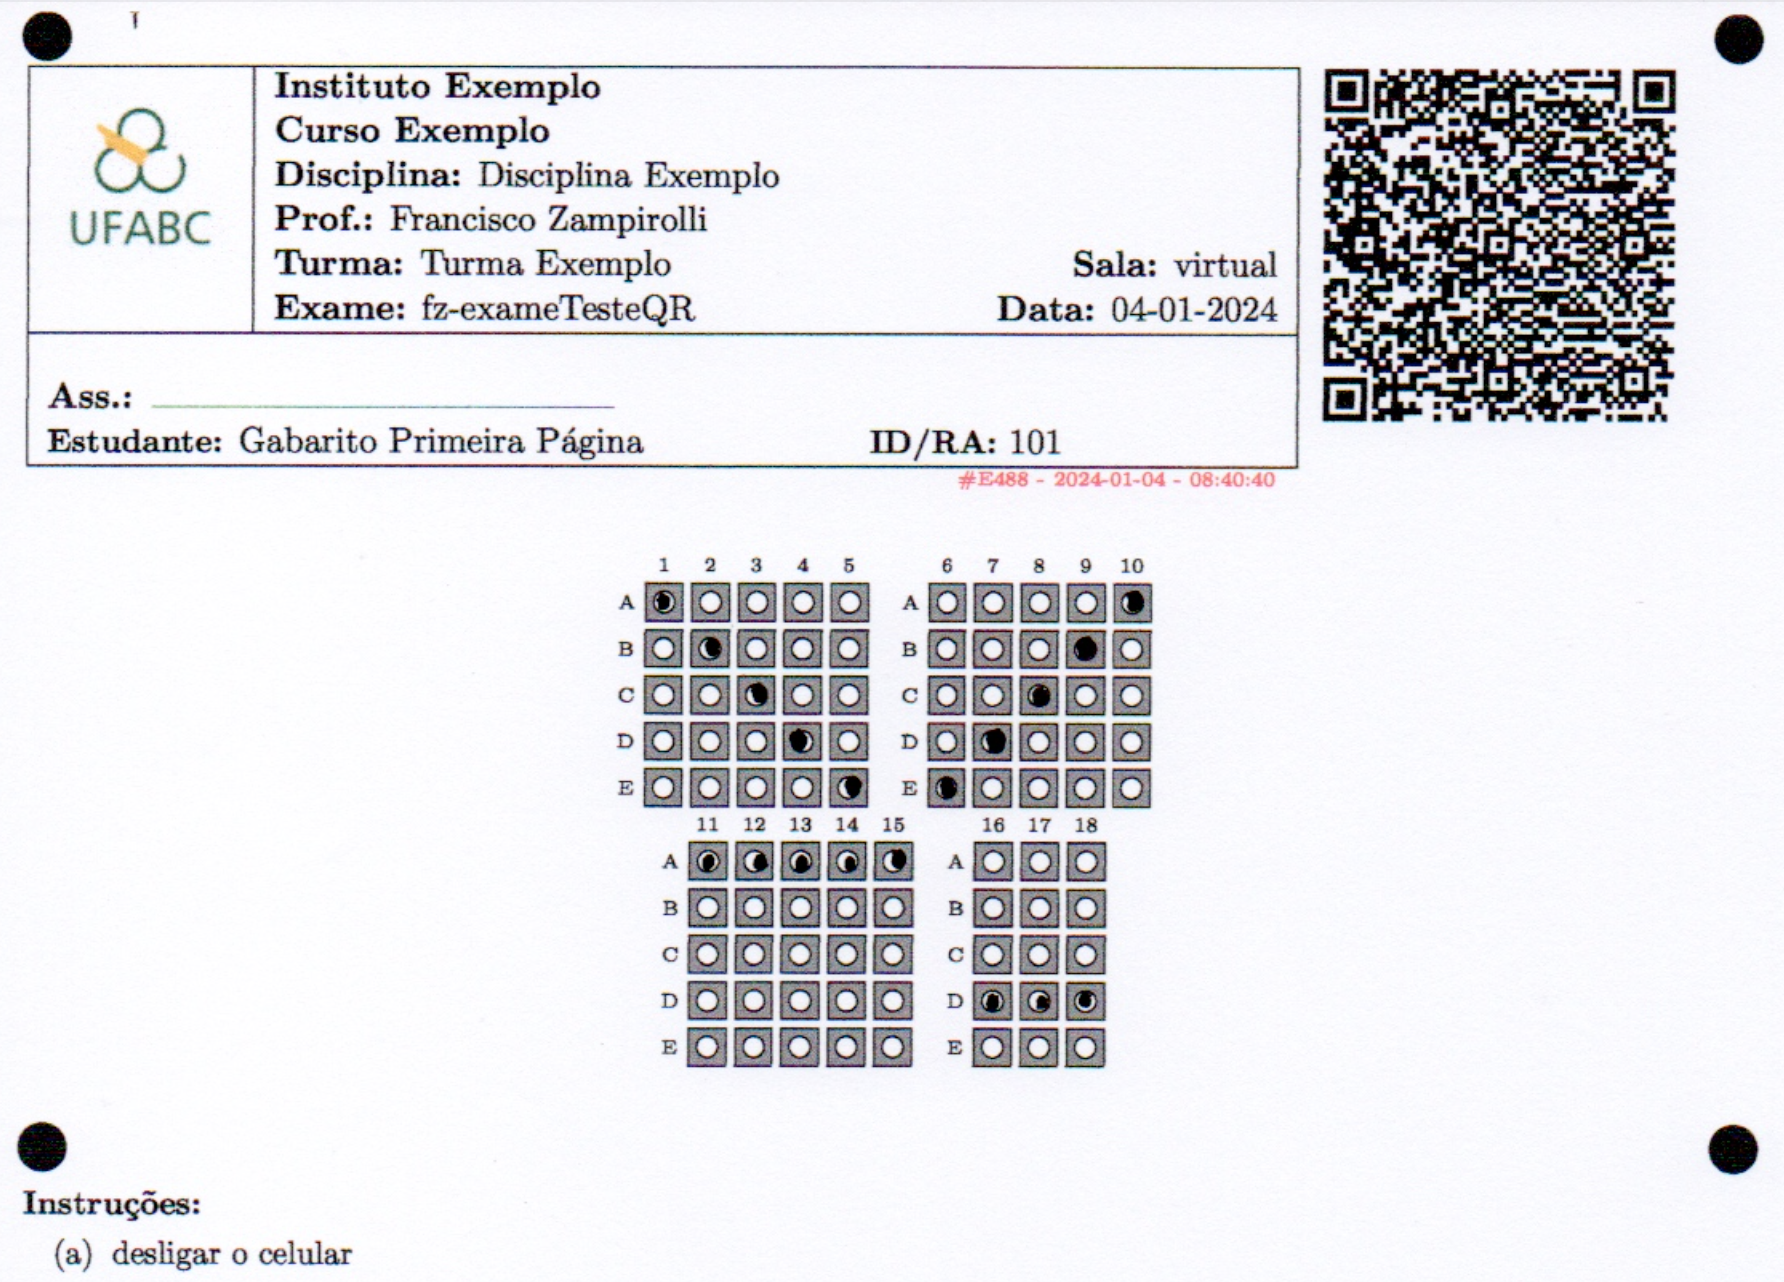
\includegraphics[width=0.54\textwidth]{cap07_figquestoesPorBlocoScan1.png}\\(a)\\
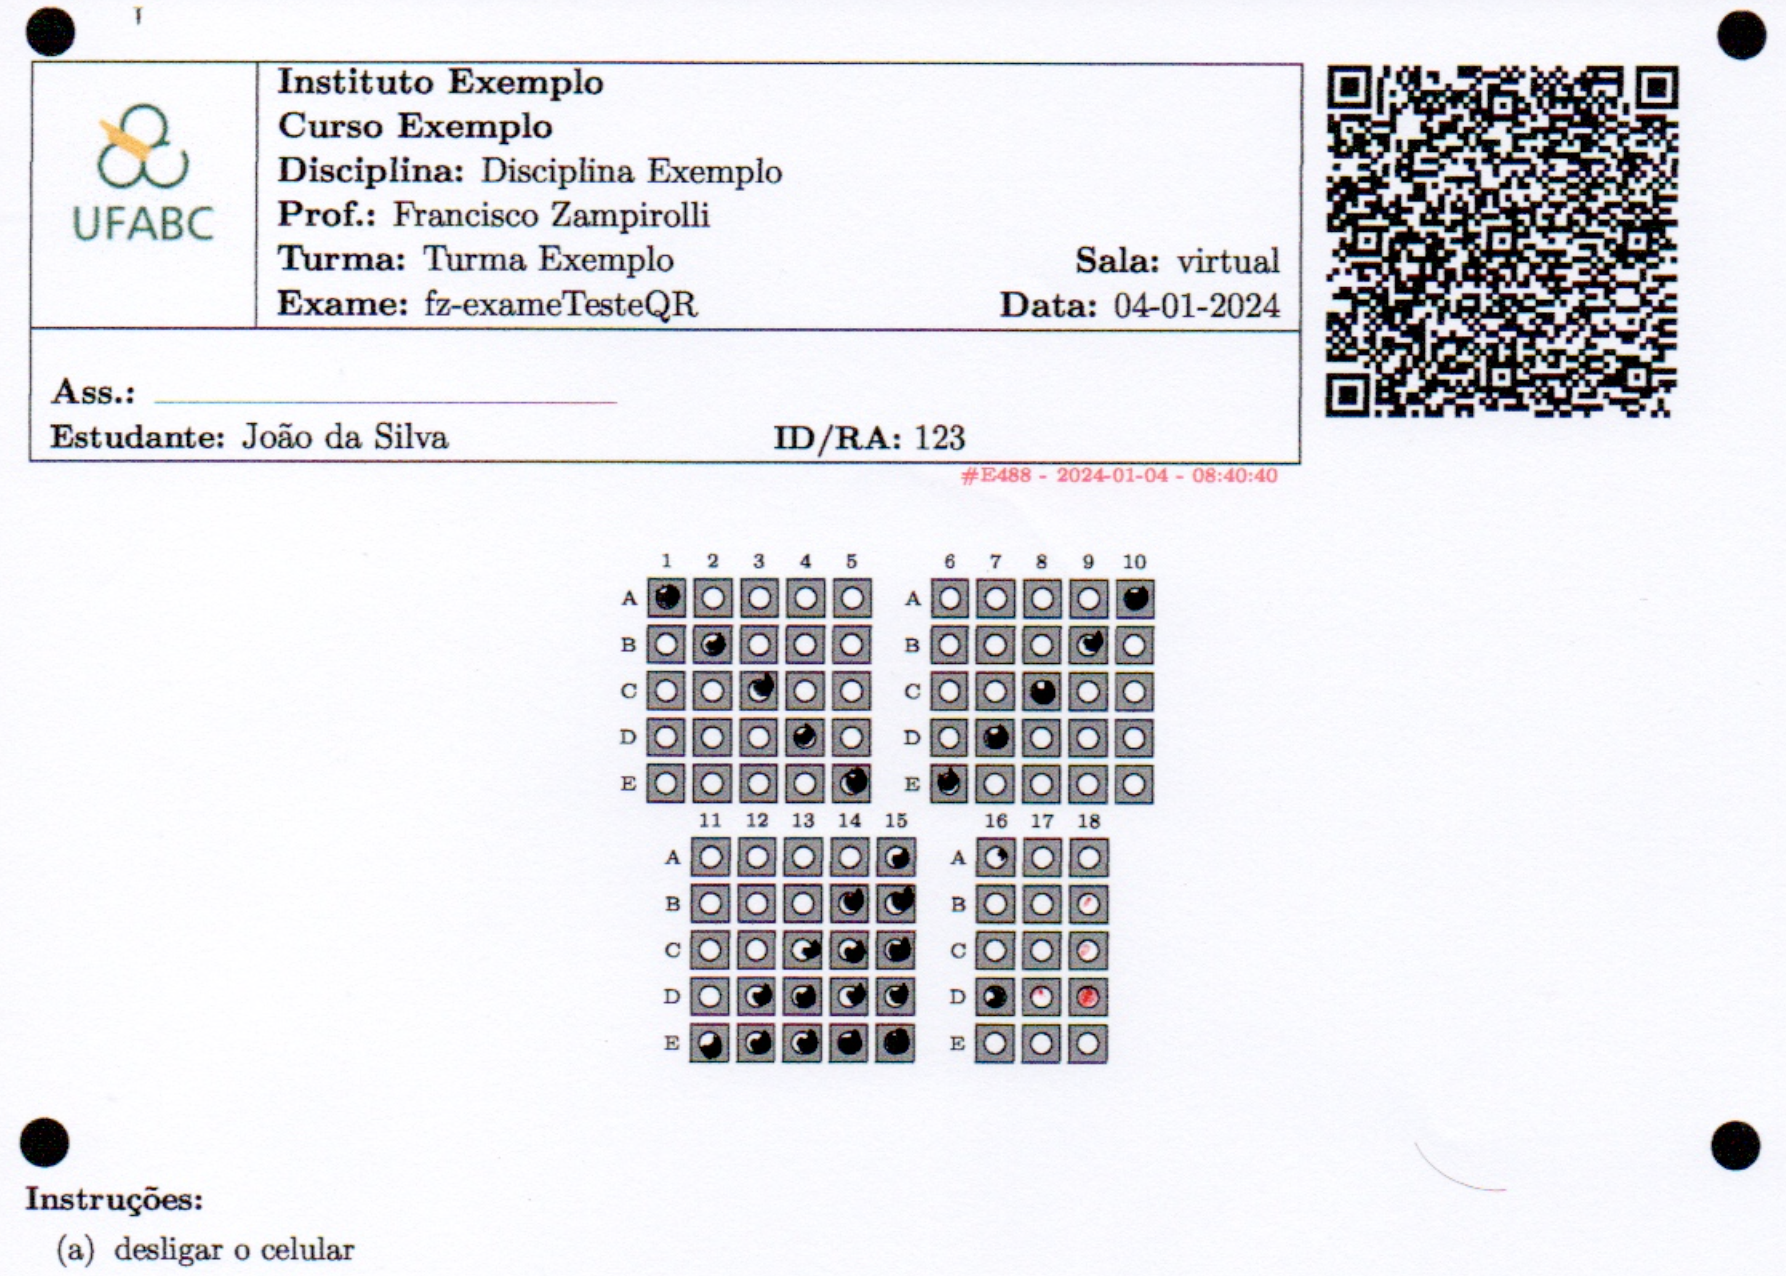
\includegraphics[width=0.54\textwidth]{cap07_figquestoesPorBlocoScan2.png}\\(b)\\
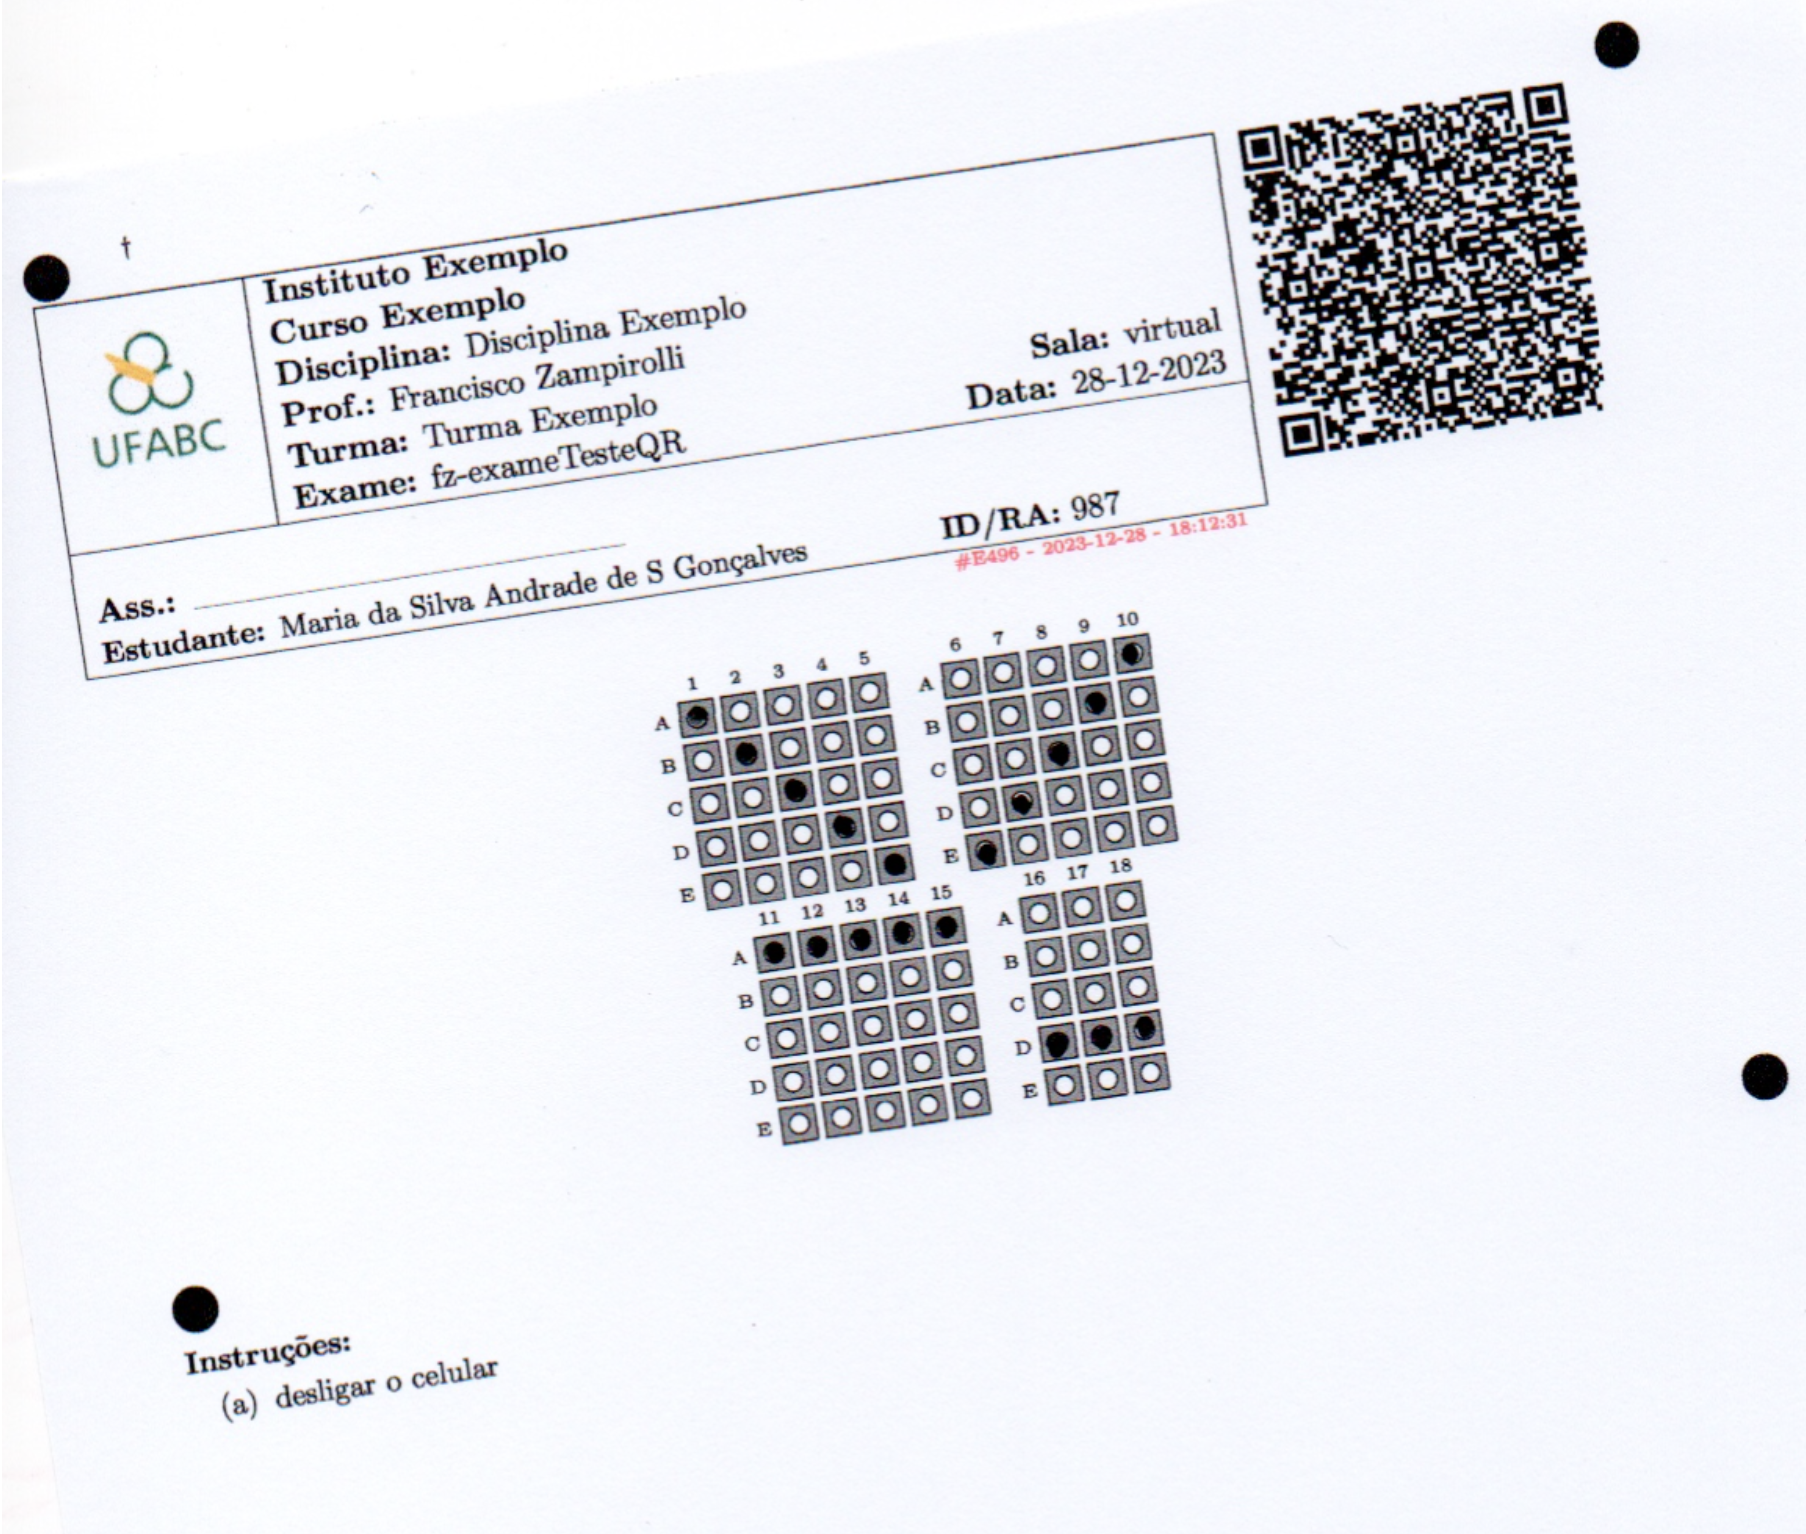
\includegraphics[width=0.54\textwidth]{cap07_figquestoesPorBlocoScan3.png}\\(c)
%(a) \hspace{7cm} (b)
\caption{Exemplos de exames digitalizados incluem: (a) o gabarito obtido a partir do PDF apresentado na Figura \ref{fig:cap07_figquestoesPorBloco}; (b) e (c) representam dois exemplos adicionais de respostas de estudantes.}
\label{fig:cap07_figquestoesPorBlocoScan}
\end{figure}

É importante mencionar que a Figura \ref{fig:cap07_figquestoesPorBlocoScan}--(c) exibe a digitalização da página rotacionada de propósito. Isso pode ser feito sem problemas com rotações inferiores a $+/- 45$ graus, desde que os quatro discos pretos externos estejam intactos na digitalização.

\begin{mybox}{corEdicao2}{\textbf{Destaque:\\\vspace{-3mm}\hrule\vspace{3mm}}}
Se algum dos quatro discos não aparecer durante a digitalização, uma sugestão seria pintar o que estiver faltando com o mesmo diâmetro e realizar uma nova digitalização. Outra opção é realizar a pintura diretamente no arquivo digitalizado, utilizando, por exemplo, a ferramenta disponível em \href{www.ilovepdf.com}{ilovepdf.com}. Lembrando que os quatro discos devem formar um retângulo imaginário com as marcações e o QRcode internos.
\end{mybox}

Após fazer o \textit{upload} deste PDF digitalizado, seguindo as instruções descritas na Seção \ref{sec:exameRecorte1} - \nameref{sec:exameRecorte1}, serão gerados vários arquivos que serão compactados em um arquivo ZIP, conforme apresentado a seguir:

\begin{myboxCode}{corCSV}{\textbf{Arquivos gerados ao solicitar a correção do exame no botão ``Upload-PDF''}}\vspace{3mm}
\hrule
\begin{verbatim}
_e488_fzampirolli@ufabc.edu.br_e488_varID_0_class_672_scan_RETURN__.csv
_e488_fzampirolli@ufabc.edu.br_e488_varID_0_class_672_scan_RETURN_p002_s3_q002.png
_e488_fzampirolli@ufabc.edu.br_e488_varID_0_class_672_scan_RETURN_p002_s3_q003.png
_e488_fzampirolli@ufabc.edu.br_e488_varID_0_class_672_scan_RETURN_p002_s3_q004.png
_e488_fzampirolli@ufabc.edu.br_e488_varID_0_class_672_scan_RETURN_p002_s3_q005.png
_e488_fzampirolli@ufabc.edu.br_e488_varID_0_class_672_scan_RETURN_p002_s4_q001_D_OK.png
_e488_fzampirolli@ufabc.edu.br_e488_varID_0_class_672_scan_RETURN_irt.csv
_e488_fzampirolli@ufabc.edu.br_e488_varID_0_class_672_scan_RETURN_statistics.csv
studentEmail_e488.zip
\end{verbatim}
\end{myboxCode}

Nesses arquivos, o prefixo \verb|_e488_| representa o ID do exame no banco de dados, seguido pelo e-mail do professor logado no MCTest e pelo nome do arquivo digitalizado e enviado para correção. O sufixo \verb|_RETURN_| indica que esses arquivos serão compactados e enviados ao e-mail do professor vinculado à conta logada no MCTest. 

\subsection{Arquivo CSV com as correções}\label{sec:CSVcorrecoesQR}

O conteúdo do primeiro arquivo CSV na lista anterior, \verb|*_.csv|, apresenta a seguinte estrutura: a primeira linha contém o cabeçalho, onde \verb|Pag| representa a página do PDF, \verb|ID| é a identificação do estudante obtida por meio do QRcode, \verb|Resp| indica a quantidade de alternativas, \verb|Quest| representa a quantidade de questões, \verb|Inv| indica as questões inválidas (sem marcação ou com mais de uma marcação), e \verb|Grade| mostra a quantidade de questões marcadas corretamente, conforme o gabarito presente na segunda linha. A segunda linha contém a compilação do gabarito (compilação da primeira página do PDF), enquanto a linha seguinte representa o exame com erros no preenchimento (compilação da segunda página do PDF). É possível observar que existem cinco questões inválidas identificadas pela coluna \verb|Inv|, correspondentes às questões de 12 a 15 do terceiro bloco (identificado como \verb|s3| na lista acima), ver Figura \ref{fig:cap07_figquestoesPorBlocoScan}--(b), além da questão 17 no quarto bloco. 

Essas questões foram salvas como arquivos PNG e estão exibidas na Figura \ref{fig:cap07_figquestoesPorBlocoScanErros}. Essas imagens são úteis, pois o professor pode analisá-las para verificar possíveis alterações na quantidade de respostas corretas do estudante. A quarta linha deste arquivo CSV corresponde à repetição do gabarito (compilação da terceira página do PDF), com exceção da marcação inválida na questão 9. 

Optou-se por não enviar os recortes das questões sem marcação ou com baixa marcação (\verb|0/*|, como mostram as questões 17 da segunda página e 9 da terceira página), pois é comum o estudante deixar questões em branco, o que geraria muitas imagens no arquivo ZIP.

\begin{myboxCode}{corCSV}{\textbf{Conteúdo do arquivo \texttt{*\_.csv} gerado (as colunas são separadas por vírgula)}}\vspace{3mm}
\hrule
{\footnotesize
\begin{verbatim}
Pag ID  Resp Quest Inv Grade Q1 Q2 Q3 Q4 Q5 Q6 Q7 Q8 Q9  Q10 Q11 Q12 Q13 Q14 Q15 Q16 Q17 Q18
1   101   5    18   0     0  A  B  C  D  E  E  D  C  B   A   A   A   A   A   A   D   D   D
2   123   5    18   6    12  A  B  C  D  E  E  D  C  B   A   E/A 2/A 3/A 4/A 5/A D   0/D D
3   987   5    17   1    17  A  B  C  D  E  E  D  C  0/B A   A   A   A   A   A   D   D   D
\end{verbatim}
}
\end{myboxCode}

\begin{mybox}{corCopia}{\textbf{Atenção:\\\vspace{-3mm}\hrule\vspace{1mm}}}
\begin{enumerate}
\item Quando ocorre um erro na decodificação do QRcode, é apresentado \verb|ERROR| na coluna \verb|Pag|;
\item Quando ocorre um erro na compilação dos QRs, como apresentados nas Figuras \ref{fig:cap07_figvertical} e \ref{fig:cap07_fighorizontal}, as colunas \verb|Resp| e \verb|Quest|  apresentam números diferentes dos definidos no formulário do exame.
\end{enumerate}
\end{mybox}

\begin{figure}[!ht]
\centering
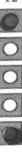
\includegraphics[width=0.05\textwidth]{cap07_figquestoes_q002.png} \ \ \ 
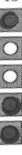
\includegraphics[width=0.053\textwidth]{cap07_figquestoes_q003.png} \ \ \ 
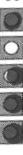
\includegraphics[width=0.053\textwidth]{cap07_figquestoes_q004.png} \ \ \ 

\includegraphics[width=0.0549\textwidth]{cap07_figquestoes_q005.png} \hspace{11mm} 
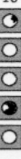
\includegraphics[width=0.053\textwidth]{cap07_figquestoes_q001_D_OK.png} \hspace{11mm} 
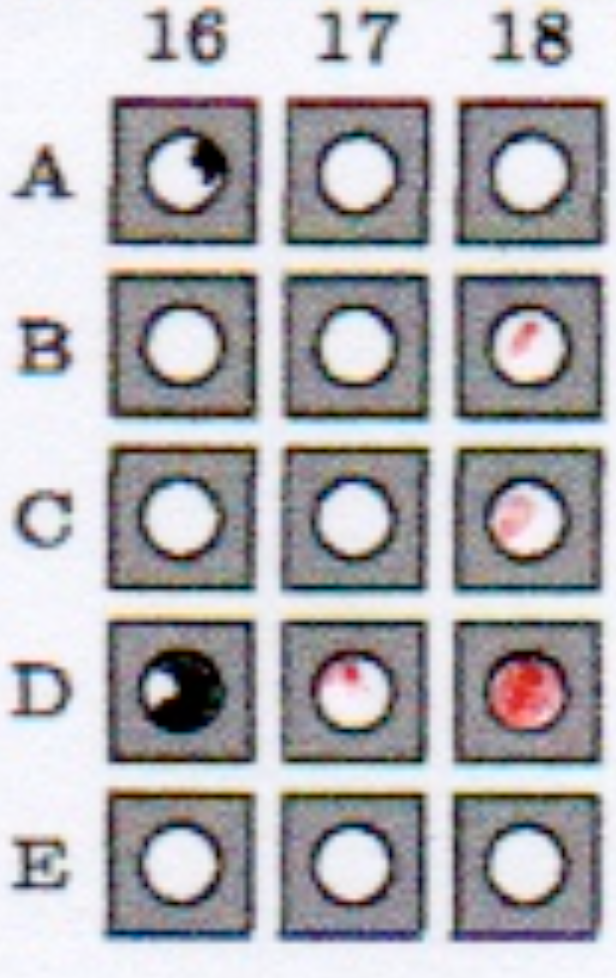
\includegraphics[width=0.27\textwidth]{cap07_figquestoes_s4.png} \ \ \ 
\caption{À esquerda, são apresentados quatro recortes automáticos das questões erroneamente marcadas no terceiro bloco, na Figura \ref{fig:cap07_figquestoesPorBlocoScan}--(b). No centro, encontra-se outro recorte automático referente ao quarto bloco, onde a alternativa D foi considerada correta. À direita, também no quarto bloco, a imagem é apresentada de forma ampliada para destacar múltiplas marcações em vermelho.}
\label{fig:cap07_figquestoesPorBlocoScanErros}
\end{figure}

\subsection{Teoria de Resposta ao Item}

O segundo arquivo CSV, com sufixo \verb|_irt.csv|, contém as respostas corretas (representadas pelo valor 1) e incorretas (representadas pelo valor 0), a partir da segunda linha (o gabarito da primeira linha é desconsiderado), conforme exemplificado a seguir. Esse arquivo será utilizado para realizar os cálculos da Teoria de Resposta ao Item (TRI) \cite{birnbaum1968some}.

\begin{myboxCode}{corCSV}{\textbf{Conteúdo do arquivo \texttt{*\_irt.csv} gerado (as colunas são separadas por vírgula)}}\vspace{3mm}
\hrule
{\footnotesize
\begin{verbatim}
1  1  1  1  1  1  1  1  1  1  0  0  0  0  0  1  0  1
1  1  1  1  1  1  1  1  0  1  1  1  1  1  1  1  1  1
\end{verbatim}
}
\end{myboxCode}

Os resultados da TRI foram adaptados do site criado por \href{http://y-okamoto-psy1949.la.coocan.jp/Python/en1/IRTLClassPyMC3/}{Yasuharu Okamoto}, utilizando a biblioteca \verb|PyMC3| do Python. A TRI é amplamente utilizada na medição de habilidades, sendo o Exame Nacional do Ensino Médio (ENEM) um exemplo conhecido dessa aplicação. No entanto, em psicologia, é comum adotar a abordagem de estágios para representar o desenvolvimento dessas habilidades. Esse modelo permite analisar dados de habilidades representadas por estágios, onde a probabilidade de uma resposta correta aumenta à medida que o estágio avança. No caso do MCTest, utilizou-se um número de estágios K=5, representando os cinco conceitos que o estudante pode alcançar (A, B, C, D e F) na graduação da UFABC. O \textit{script} adaptado calcula as probabilidades de respostas corretas entre esses estágios.

Ao detalhar um pouco mais esse processo, é importante mencionar que o MCTest calcula automaticamente a TRI de cada PDF digitalizado submetido para correção. No entanto, para calcular a TRI dos 2553 candidatos que participaram do processo seletivo da EPUFABC em 2019, foi necessário reunir todos esses arquivos \verb|_irt.csv| obtidos dos PDFs submetidos em um único arquivo. Para otimizar o tempo de processamento, realizou-se a ordenação e criou-se um novo CSV contendo os dados dos 1000 candidatos com melhor classificação. Em seguida, utilizou-se o \textit{script} disponibilizado no GitHub, no arquivo \href{https://github.com/fzampirolli/mctest/blob/master/_irt_pymc3_shell.py}{\texttt{github.com/fzampirolli/mctest/blob/master/\_irt\_pymc3\_shell.py}}. Especificamente para o trabalho de \citeonline{2021:Zampirolli.Batista.ea}, foi utilizada também a linguagem de programação R para processar todos os candidatos.

\begin{mybox}{pink}{\textbf{Melhorias:\\\vspace{-3mm}\hrule}\vspace{3mm}}
Para trabalhos futuros, é necessário adaptar esse processo de cálculo da TRI para lidar de forma mais eficiente com um número maior de candidatos, visto que a abordagem atual se limita aos 1000 mais bem classificados.
\end{mybox}



Os resultados obtidos por meio da TRI serão apresentados no terceiro arquivo CSV, com sufixo \verb|_statistics.csv|, conforme demonstrado a seguir. Nesse arquivo de estatísticas, a primeira coluna, \verb|id|, representa o número da questão. A coluna \verb|corr| indica o número de respostas corretas, enquanto a coluna \verb|fail| indica o número de respostas marcadas incorretamente. A coluna \verb|aver| representa a média de acertos, e a coluna \verb|str| indica o desvio padrão. Em seguida, têm-se as colunas \verb|%corr| e \verb|%fail|, que representam a porcentagem de respostas corretas e incorretas, respectivamente.

No entanto, é importante ressaltar que um experimento completo realizado na EPUFABC, que resultou no trabalho de \citeonline{2021:Zampirolli.Batista.ea}, será apresentado na parte de experimentos deste livro.

\begin{myboxCode}{corCSV}{\textbf{Conteúdo do arquivo \texttt{*\_statistics.csv} gerado (as colunas são separadas por vírgula)}}\vspace{3mm}
\hrule
{\footnotesize
\begin{verbatim}
id corr fail aver std  %corr %fail
 1   2   0   1.0  0.0   1.0   0.0
 2   2   0   1.0  0.0   1.0   0.0
 3   2   0   1.0  0.0   1.0   0.0
 4   2   0   1.0  0.0   1.0   0.0
 5   2   0   1.0  0.0   1.0   0.0
 6   2   0   1.0  0.0   1.0   0.0
 7   2   0   1.0  0.0   1.0   0.0
 8   2   0   1.0  0.0   1.0   0.0
 9   1   1   0.5  0.5   0.5   0.5
10   2   0   1.0  0.0   1.0   0.0
11   1   1   0.5  0.5   0.5   0.5
12   1   1   0.5  0.5   0.5   0.5
13   1   1   0.5  0.5   0.5   0.5
14   1   1   0.5  0.5   0.5   0.5
15   1   1   0.5  0.5   0.5   0.5
16   2   0   1.0  0.0   1.0   0.0
17   1   1   0.5  0.5   0.5   0.5
18   2   0   1.0  0.0   1.0   0.0
\end{verbatim}
}
\end{myboxCode}

\subsection{\textit{Feedback} ao estudante}


Se a opção ``Retorno=Sim'' na Seção \ref{sec:exameDetalhes} -- \nameref{sec:exameDetalhes} for selecionada, ao clicar em ``Upload--PDF'', as correções do exame de cada estudante serão enviadas por e-mail em formato PDF, conforme apresentado na Figura \ref{fig:cap07_figFeedback}. É possível observar que as marcações incorretas são indicadas por um círculo na alternativa correta. No final do PDF, é fornecido um resumo contendo os dados do estudante e a quantidade de acertos. No próximo capítulo, serão apresentados mais exemplos de QR que incluem as QMs.

\begin{figure}[htbp]
  \centering
  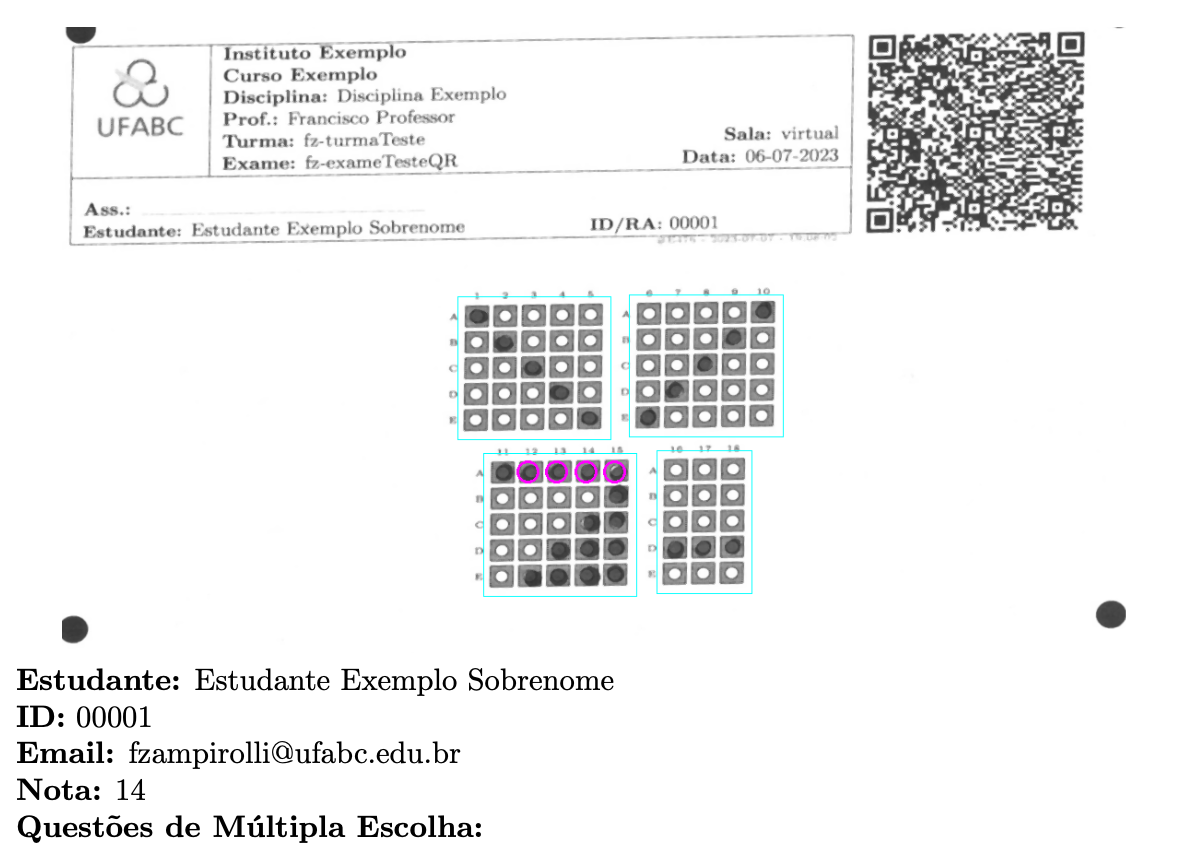
\includegraphics[width=0.9\textwidth]{cap07_figFeedback.png}
    \caption{PDF com o \textit{feedback} das correções enviado para o e-mail do estudante.}
\label{fig:cap07_figFeedback}
\end{figure}

\begin{mybox}{pink}{\textbf{Melhorias:\\\vspace{-3mm}\hrule}\vspace{3mm}}
  Na Figura \ref{fig:cap07_figFeedback}, ainda é necessário ajustar os discos vermelhos nas alternativas corretas que o estudante errou. Além disso, é necessário corrigir a apresentação da nota do estudante.
\end{mybox}

% melhorar escrita formal e científica, mantendo a formatação LaTex: 

\section{Considerações finais}

Este capítulo abordou a criação de exames exclusivamente com o QR, uma prática comumente adotada na Escola Preparatória da UFABC (EPUFABC) para processos seletivos e simulados que envolvem inúmeros estudantes anualmente. Foi demonstrado como acomodar centenas de questões em uma única página no formato PDF, que pode ser impressa e distribuída aos estudantes para preencherem manualmente as respostas.

Em seguida, os QRs são digitalizados e enviados ao MCTest para correção. O sistema envia ao professor um e-mail contendo arquivos CSV com as marcações de cada estudante e as respostas corretas. Além disso, o MCTest fornece uma síntese da Teoria de Respostas ao Item (TRI) com base nas correções realizadas. O gabarito, ou seja, as respostas corretas, é fornecido na primeira página do PDF digitalizado, que pode conter as respostas de todos os estudantes de uma turma em sequência.

Ao utilizar exames exclusivamente com QR, é importante configurar corretamente os detalhes do exame, como o número de questões, o número de alternativas por questão e o estilo do exame (horizontal ou vertical). Foi destacado que é possível corrigir eventuais erros de marcação utilizando ferramentas de edição de PDF, mas é necessário ter cuidado para preservar as marcações corretas.

Por fim, foi apresentada a possibilidade de fornecer \textit{feedback} aos estudantes, através da opção ``Retorno=Sim'' no MCTest. Nesse caso, o sistema envia por e-mail um PDF com as correções do exame para cada estudante, contendo marcações incorretas indicadas por círculos na alternativa correta, bem como um resumo dos dados do estudante e a quantidade de acertos.

No próximo capítulo, serão apresentados mais exemplos de QR que incluem as questões, ampliando as possibilidades de utilização dessa abordagem no contexto educacional.

















